\chapter{Usage}
\label{chap:usage}

Conlangtionary is, fundamentally, a tool for language development. As such, there are specific actions that a user can take within the platform to develop a language. This chapter serves as a walkthrough for the basic operations of using Conlangtionary.

\section{Accessing Conlangtionary}
\label{sec:accessing-conlangtionary}

At the time of writing, there was a running instance of Conlangtionary available on Heroku cloud hosting (see Section \ref{sec:hosting}) available at \url{conlangtionary.herokuapp.com}. The server is slow, so it could take up to 30 seconds for the page to load. This latency is a result of the server being asleep. After a user establishes a connection, it should be significantly more responsive. When the page does load, the view should be similar to Figure \ref{fig:home-not-logged-in}. Conlangtionary allows any user to view content, which is demonstrated in Section \ref{sec:exploring-conlangs}, but only authenticated users can create or edit content (see Section \ref{sec:account-registration}).

\begin{figure}[h]
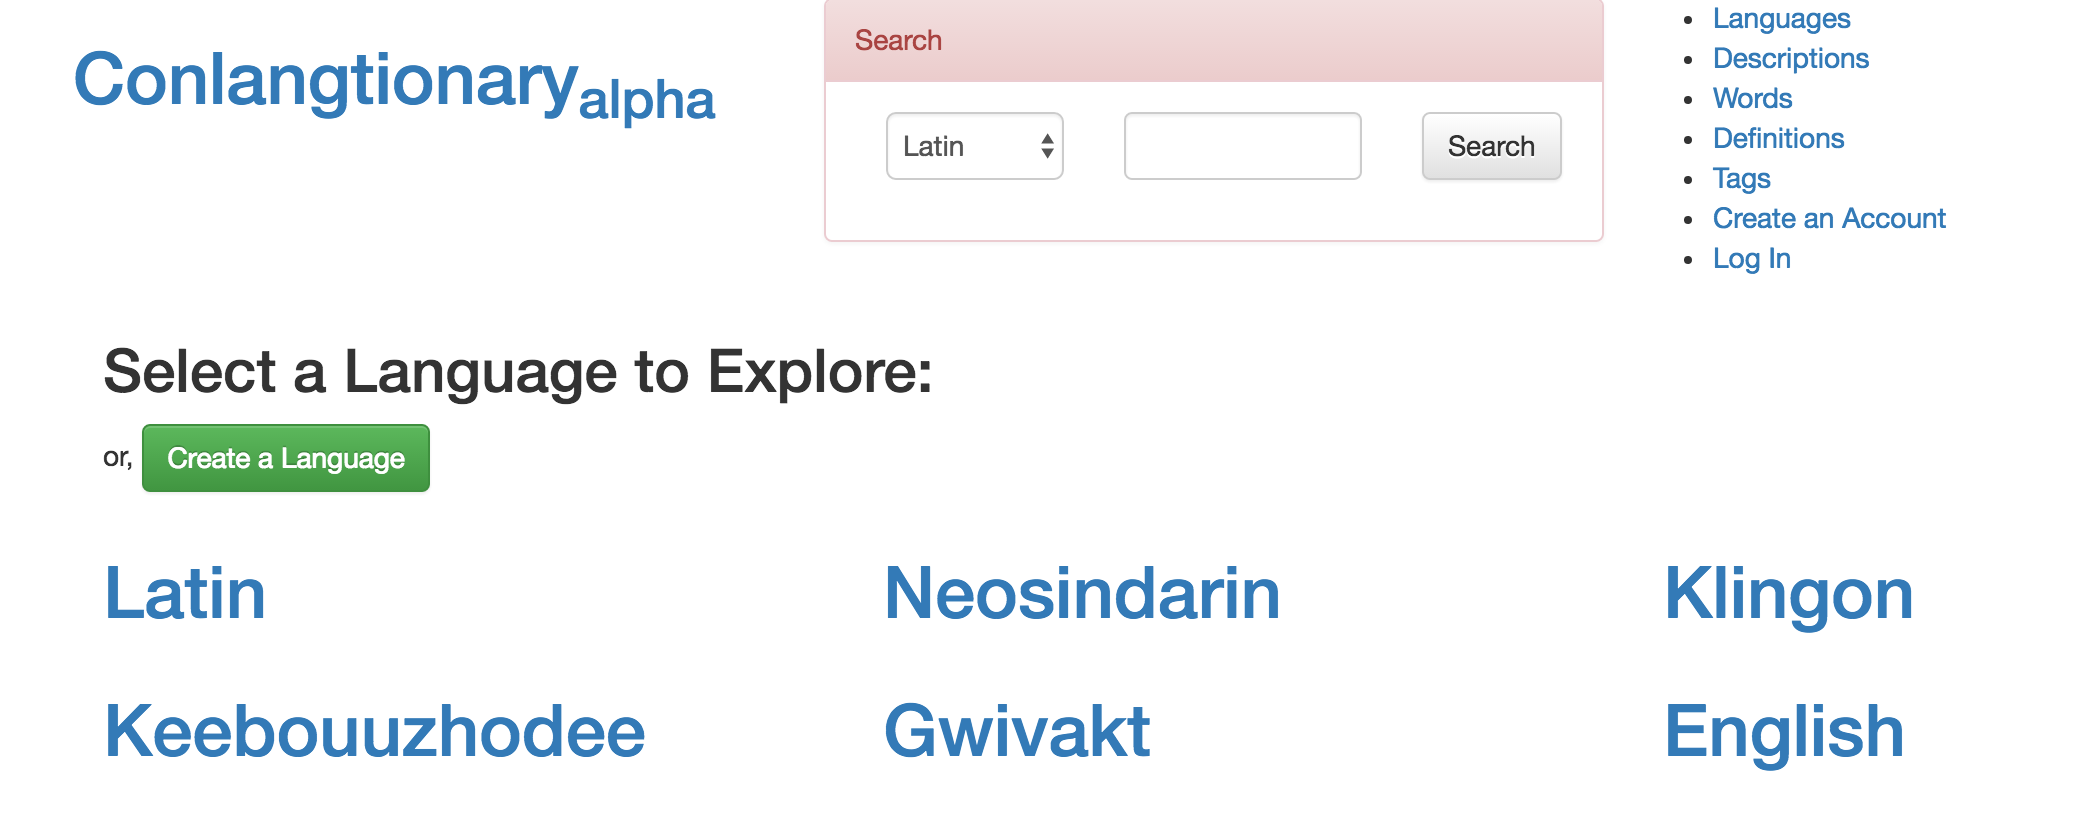
\includegraphics[width=\textwidth]{figures/home-not-logged-in}
\caption{The Conlangtionary Home Page (not logged in).}
\centering
\label{fig:home-not-logged-in}
\end{figure}

\section{Exploring Conlangs}
\label{sec:exploring-conlangs}

To explore a conlang, a user simply needs to click on its name on the home page (the page in Figure \ref{fig:home-not-logged-in}). To return to the home page, a user can just click the site's title (the $Conlangtionary_{alpha}$ in the upper-left of every page).

Every conlang has a page similar to the one depicted in Figure \ref{fig:keebouuzhodee-not-logged-in}. The page is divided into four colored content areas. It is important to note that the color of the area does not have any significance other than distinguishing sections easily. The green section hosts the language's name along with a sentence-length description and any language-level user notes. The yellow area houses all of the language's tags (see Section \ref{subsec:tags}). The blue is the language's description (see Section \ref{subsec:descriptions}). Finally, the red area houses each word with all of that word's definitions listed beneath the word (see Sections \ref{subsec:words} and \ref{subsec:definitions}).

\begin{figure}[!h]
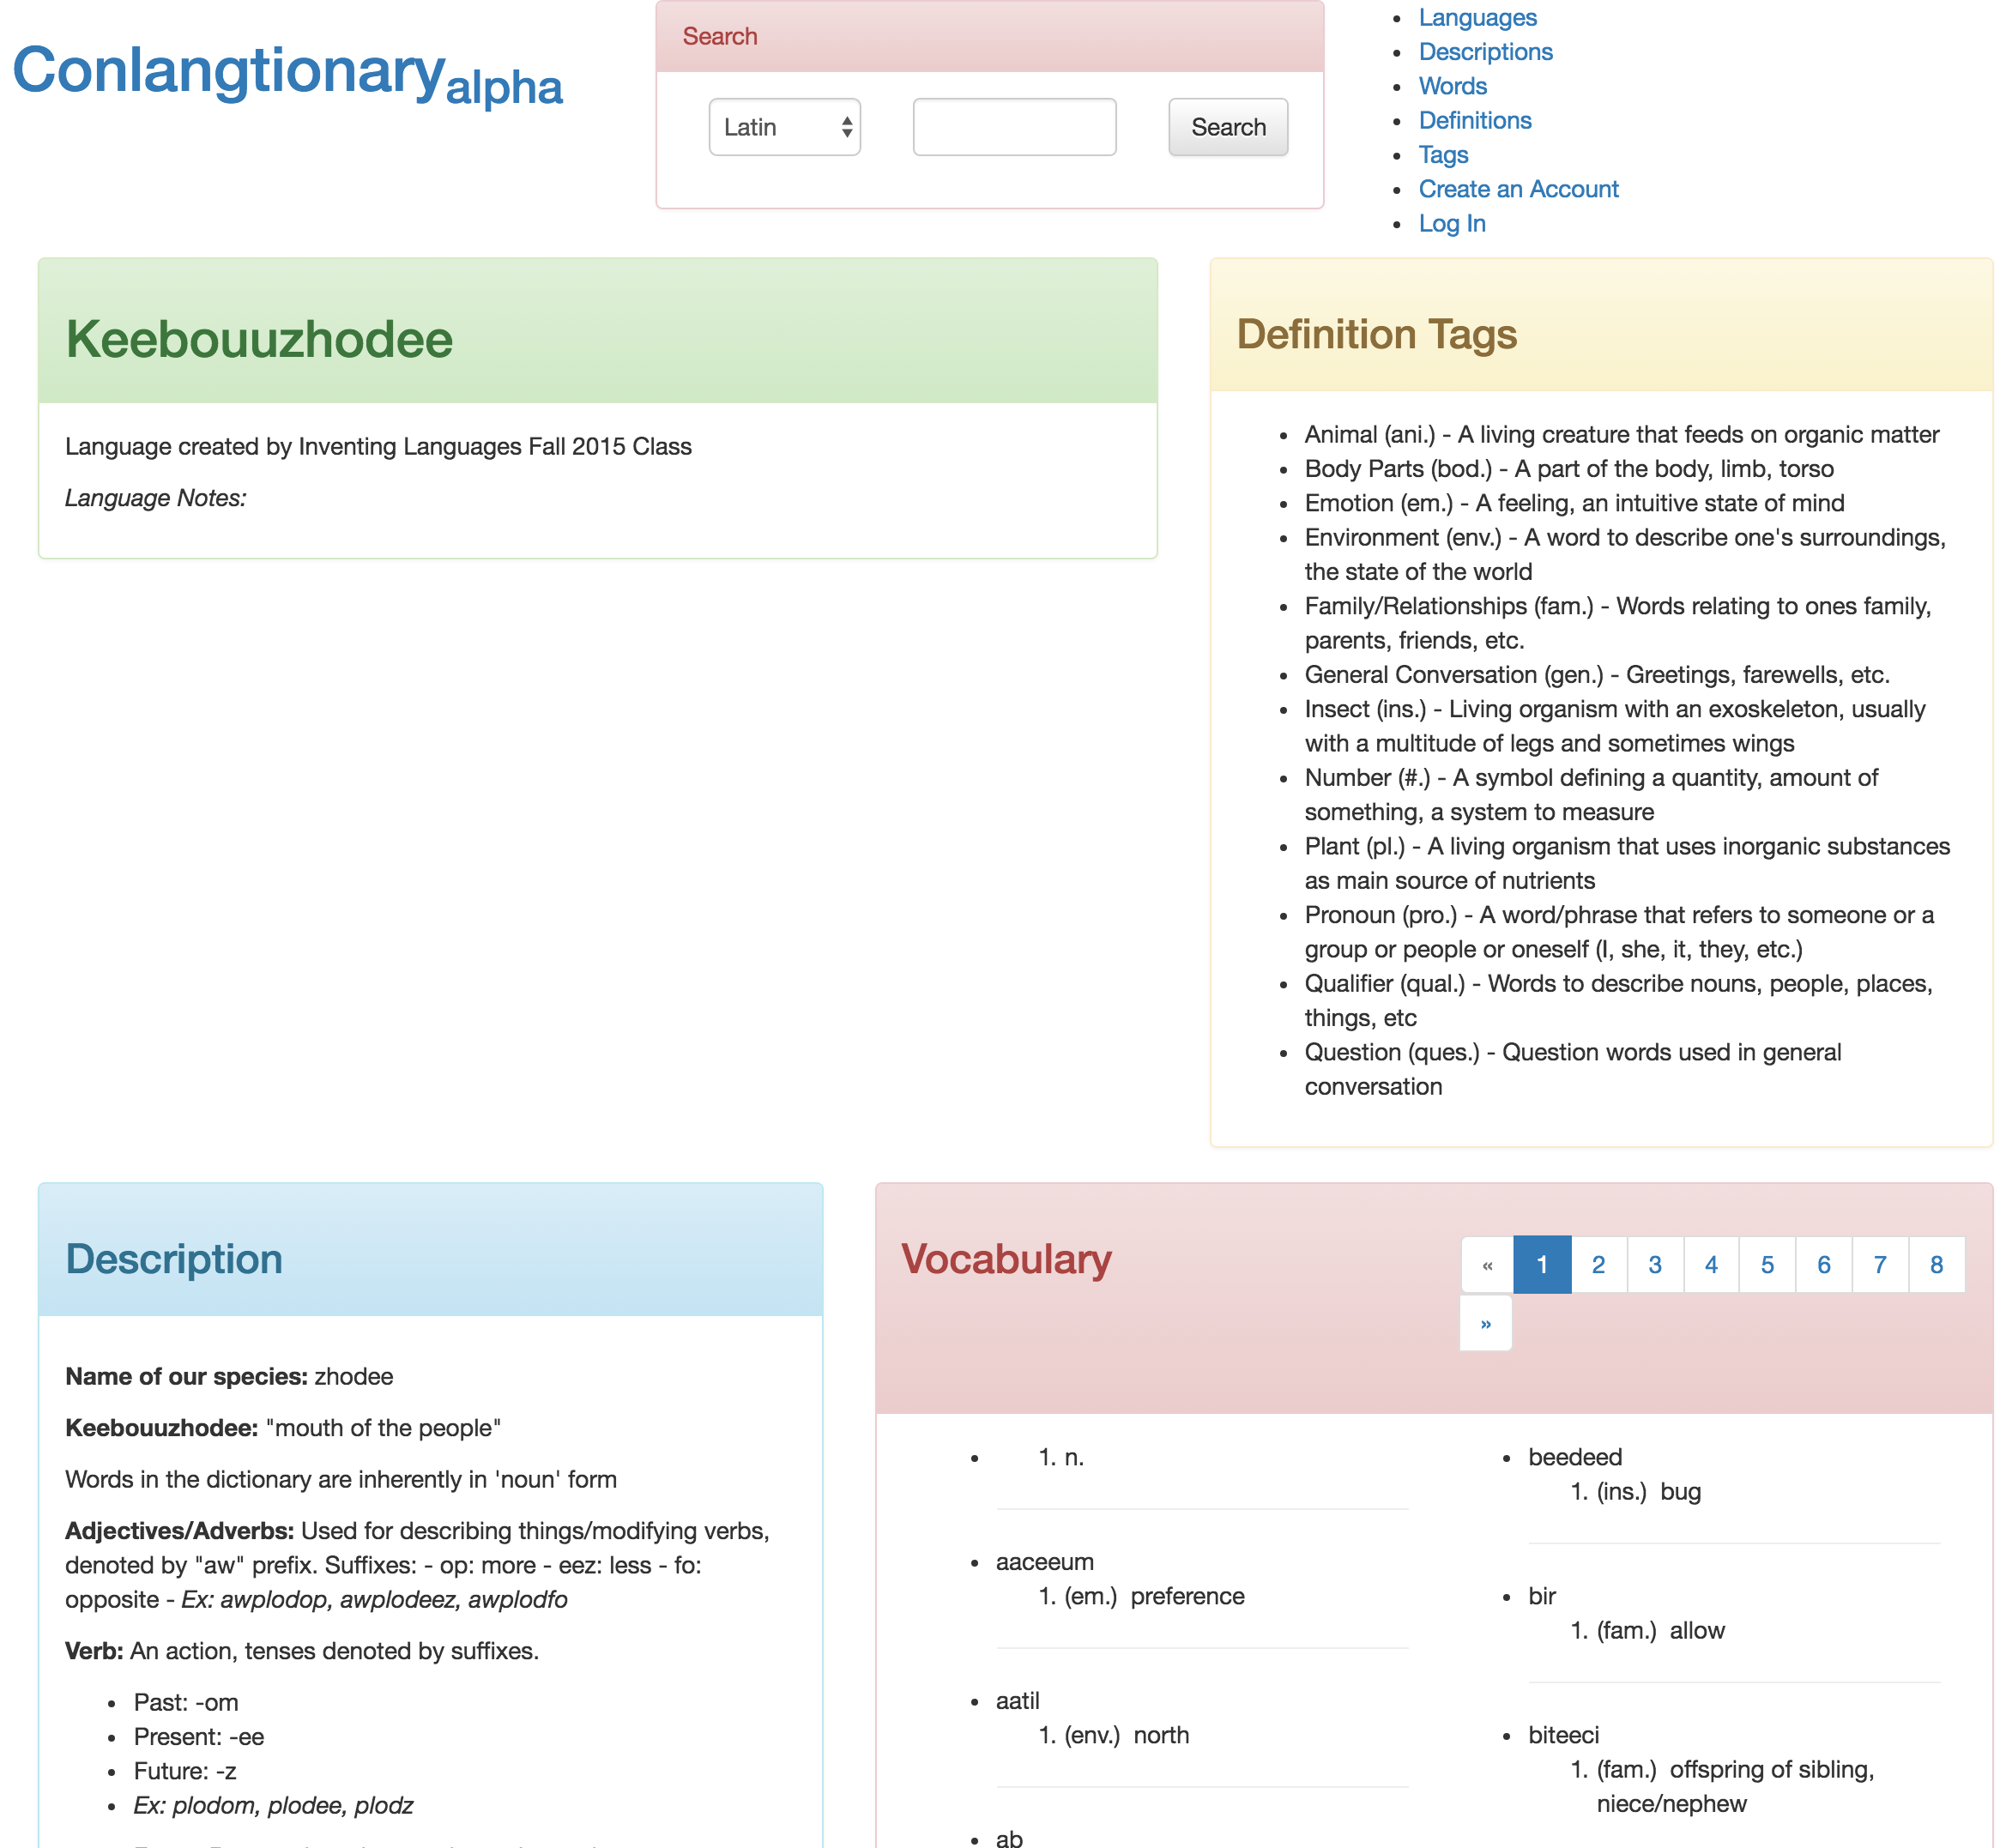
\includegraphics[width=\textwidth]{figures/keebouuzhodee-not-logged-in}
\caption{The Keebouuzhodee Language Page (not logged in).}
\centering
\label{fig:keebouuzhodee-not-logged-in}
\end{figure}

Generally, the description of a language will include a rough summary of the language's grammar and usage. It might also include external links to resources on the language hosted elsewhere. To get a feel for a language, it is best to look at the grammar and usage examples, and then to play around with the vocabulary.

The words in the red area are formatted in deliberate imitation of a dictionary. Each word has definitions listed below it, and those definitions begin with the abbreviations for every tag present on that definition. This means that if a language tags words by part of speech, words will appear with their part of speech before their definition (much like English dictionaries currently do). Every tag shows its abbreviation after its name in the yellow area, so it should be easy for users to figure out what the tags on a definition mean from this page.

\section{Account Registration}
\label{sec:account-registration}

Signing up for Conlangtionary is easy. When a user is not logged in, all they have to do is click on the ``Create an Account" link on the top right of the screen. This takes them to the page depicted in Figure \ref{fig:registration-form}. 

\begin{figure}[!h]
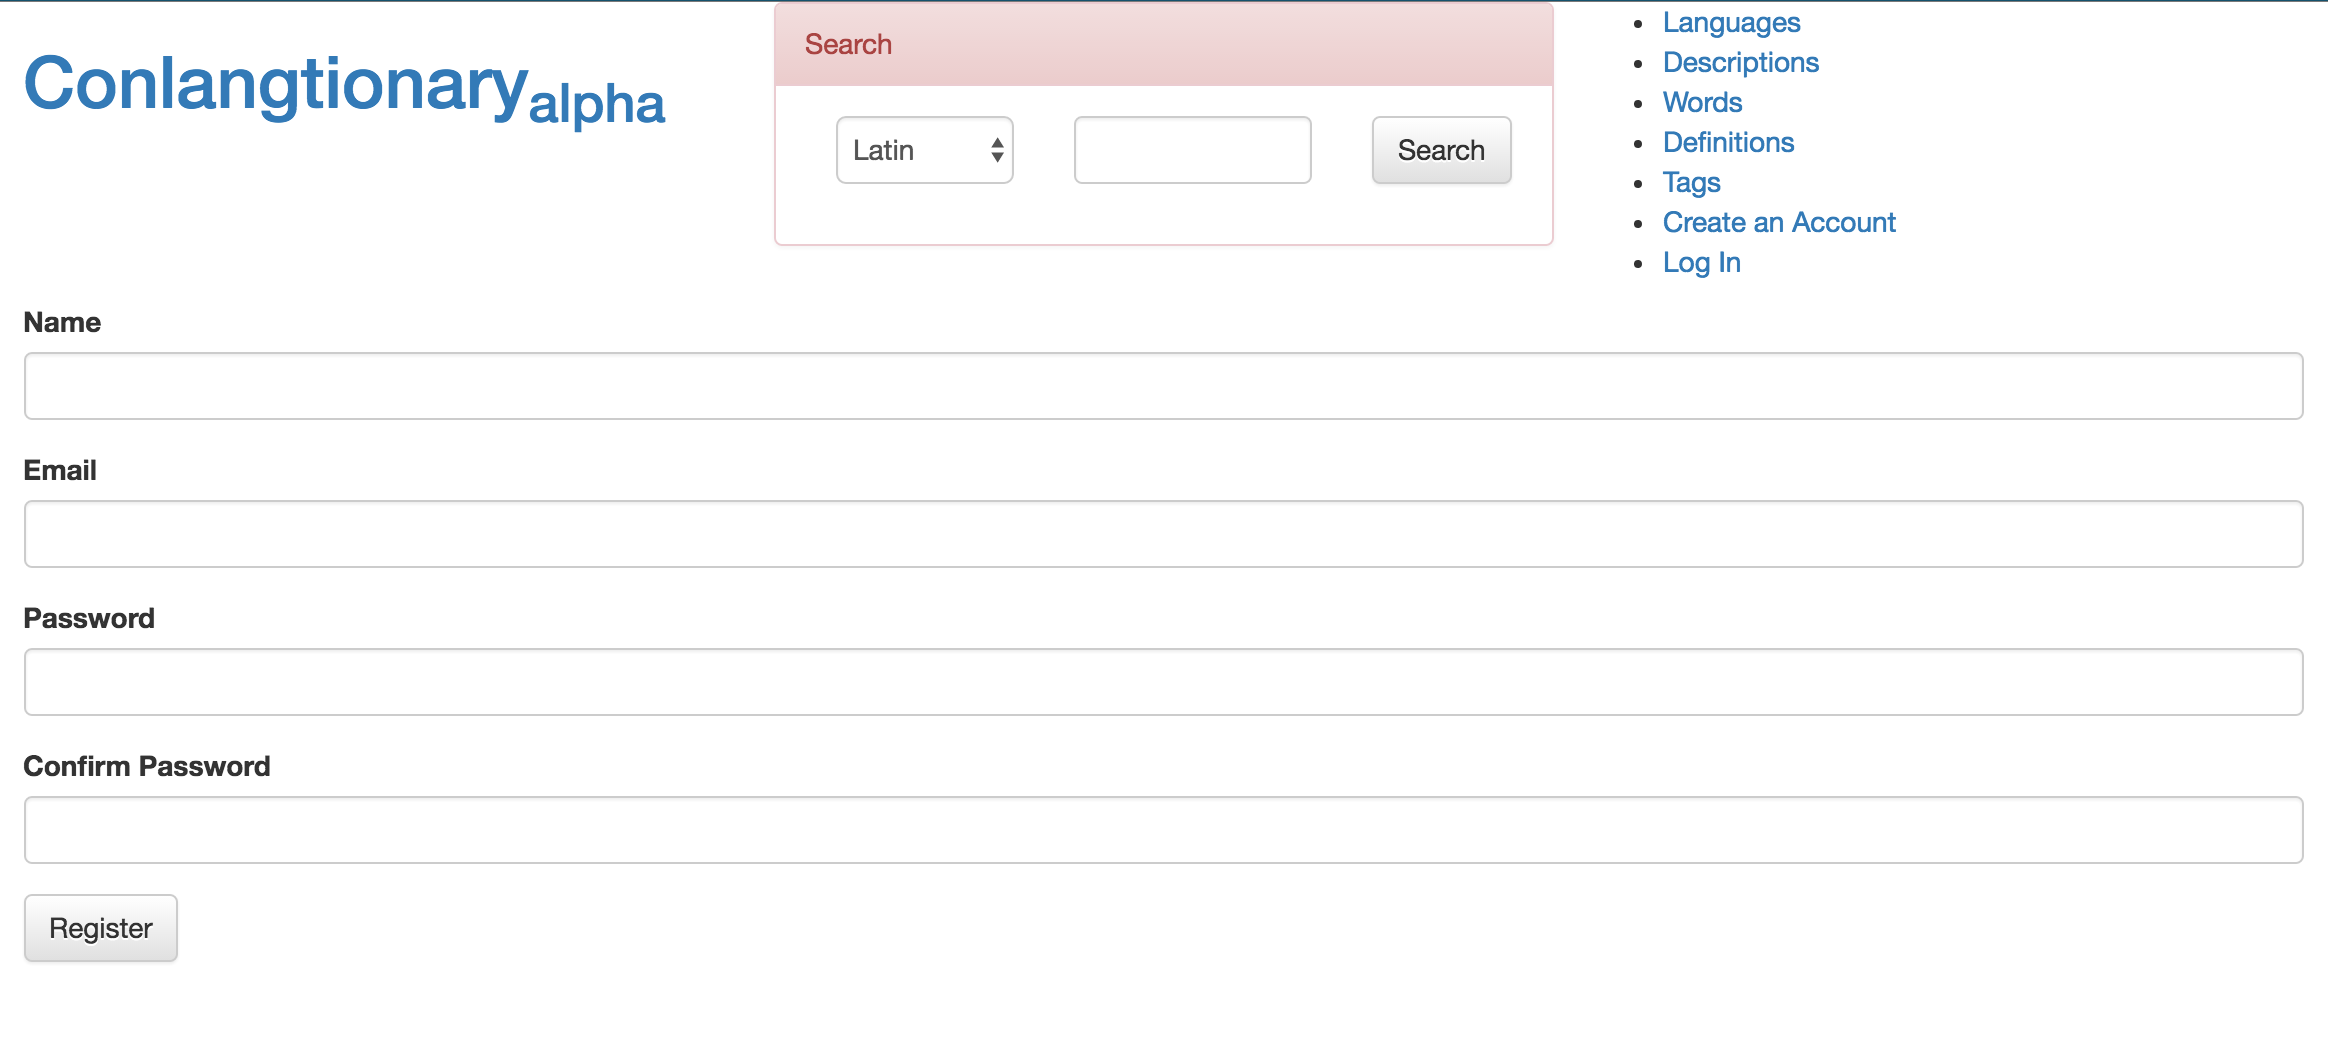
\includegraphics[width=\textwidth]{figures/registration-form}
\caption{The registration form.}
\centering
\label{fig:registration-form}
\end{figure}

Filling out this form creates a user account that can log in with the given username and password combination. There isn't currently any email validation, which does leave the site vulnerable to spam accounts. Once a user has an account, they can just click the ``Log In" link in the future to access the protected features of the site.

\section{Logging In}
\label{sec:logging-in}

\begin{figure}[h]
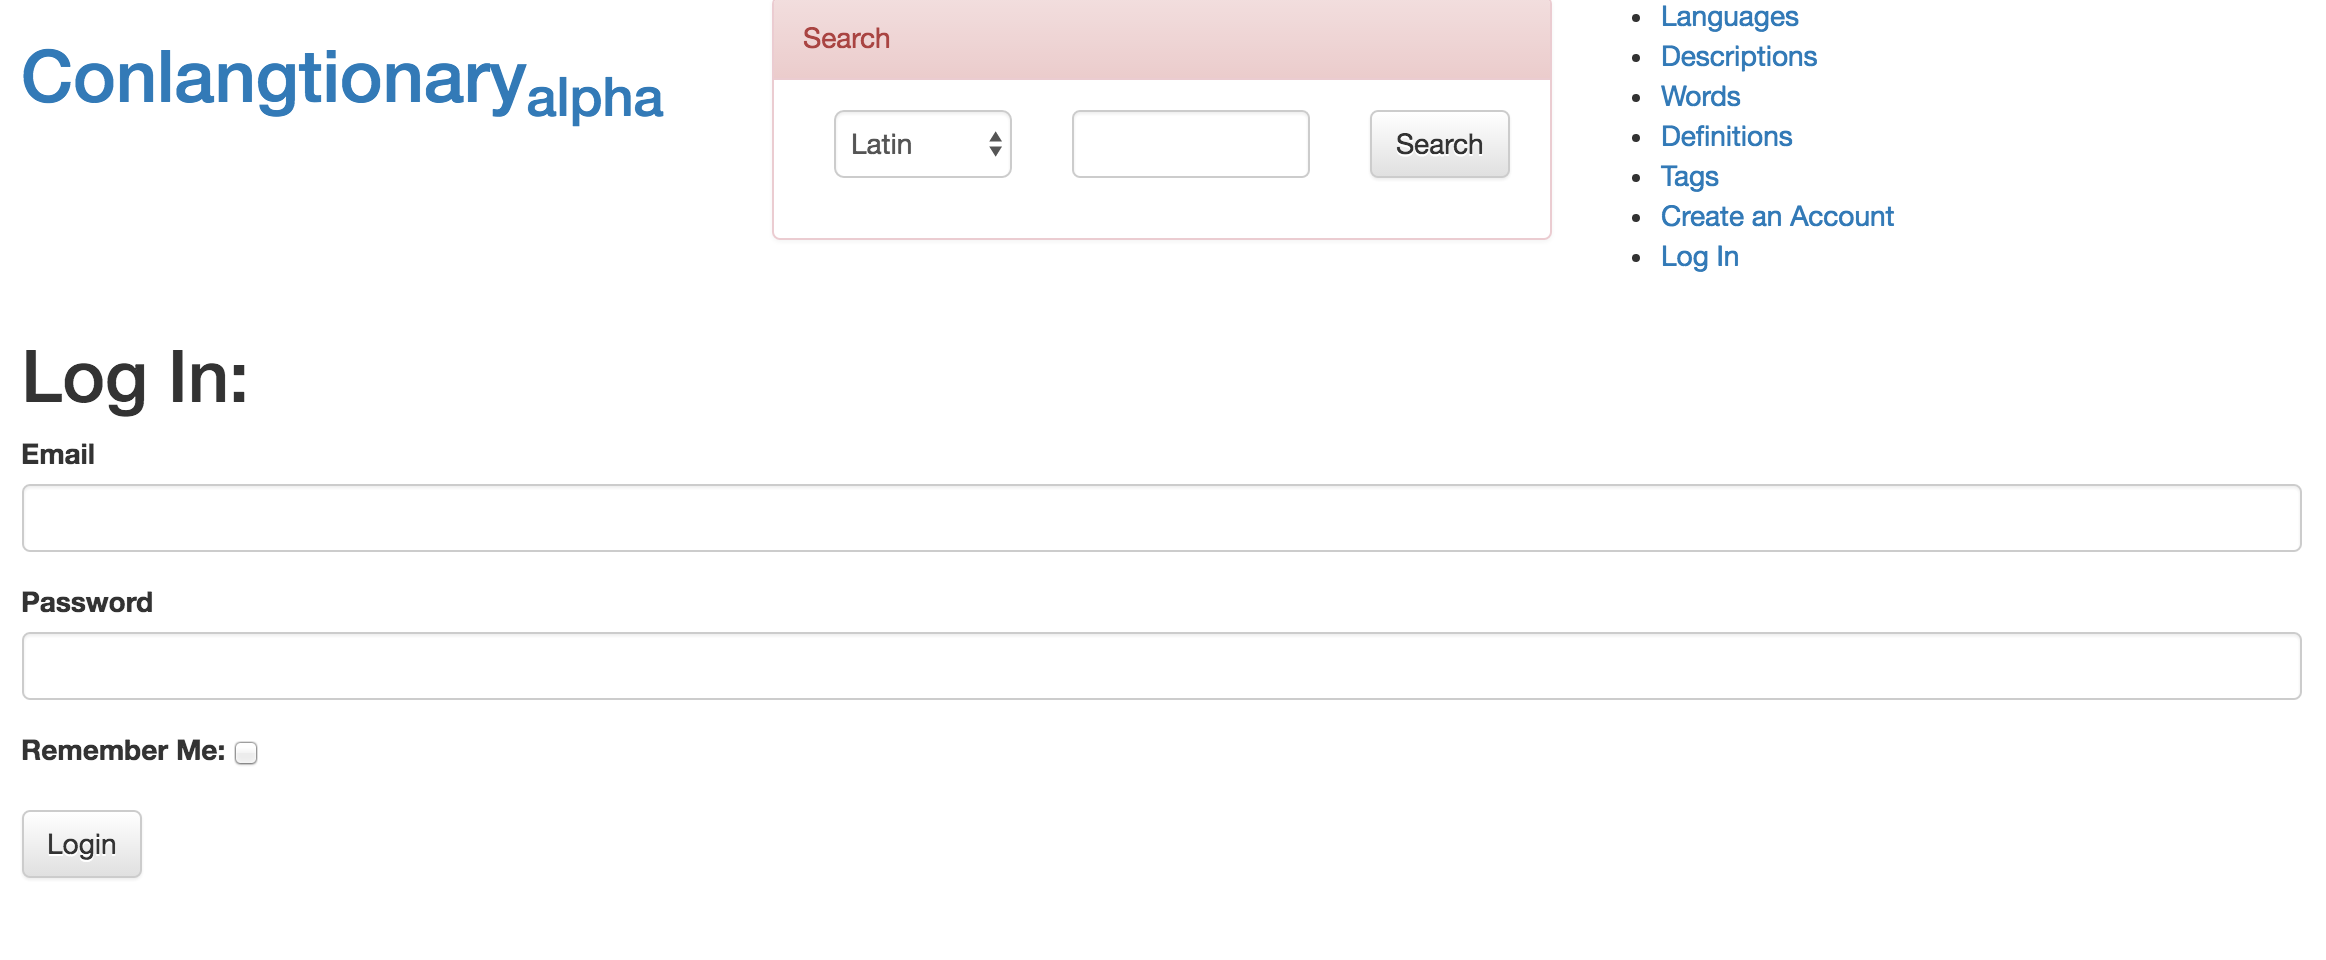
\includegraphics[width=\textwidth]{figures/log-in}
\caption{The login form.}
\centering
\label{fig:log-in}
\end{figure}

Logging into Conlangtionary is simple. Clicking the ``Log In" button in the menu takes a user to the form shown in Figure \ref{fig:log-in}. Filling out a valid email and password combination allows a user into the site.

\section{Creating a Language}
\label{sec:creating-language}

Getting started in Conlangtionary requires a language to work on. There is a button on the home screen labeled ``Create a Language" that begins the process of building a conlang. If a user is not logged in, the button will redirect to a login screen before allowing the user to proceed. The form for creating a language is simple, and can be seen in Figure \ref{fig:create-language}.

\begin{figure}[h]
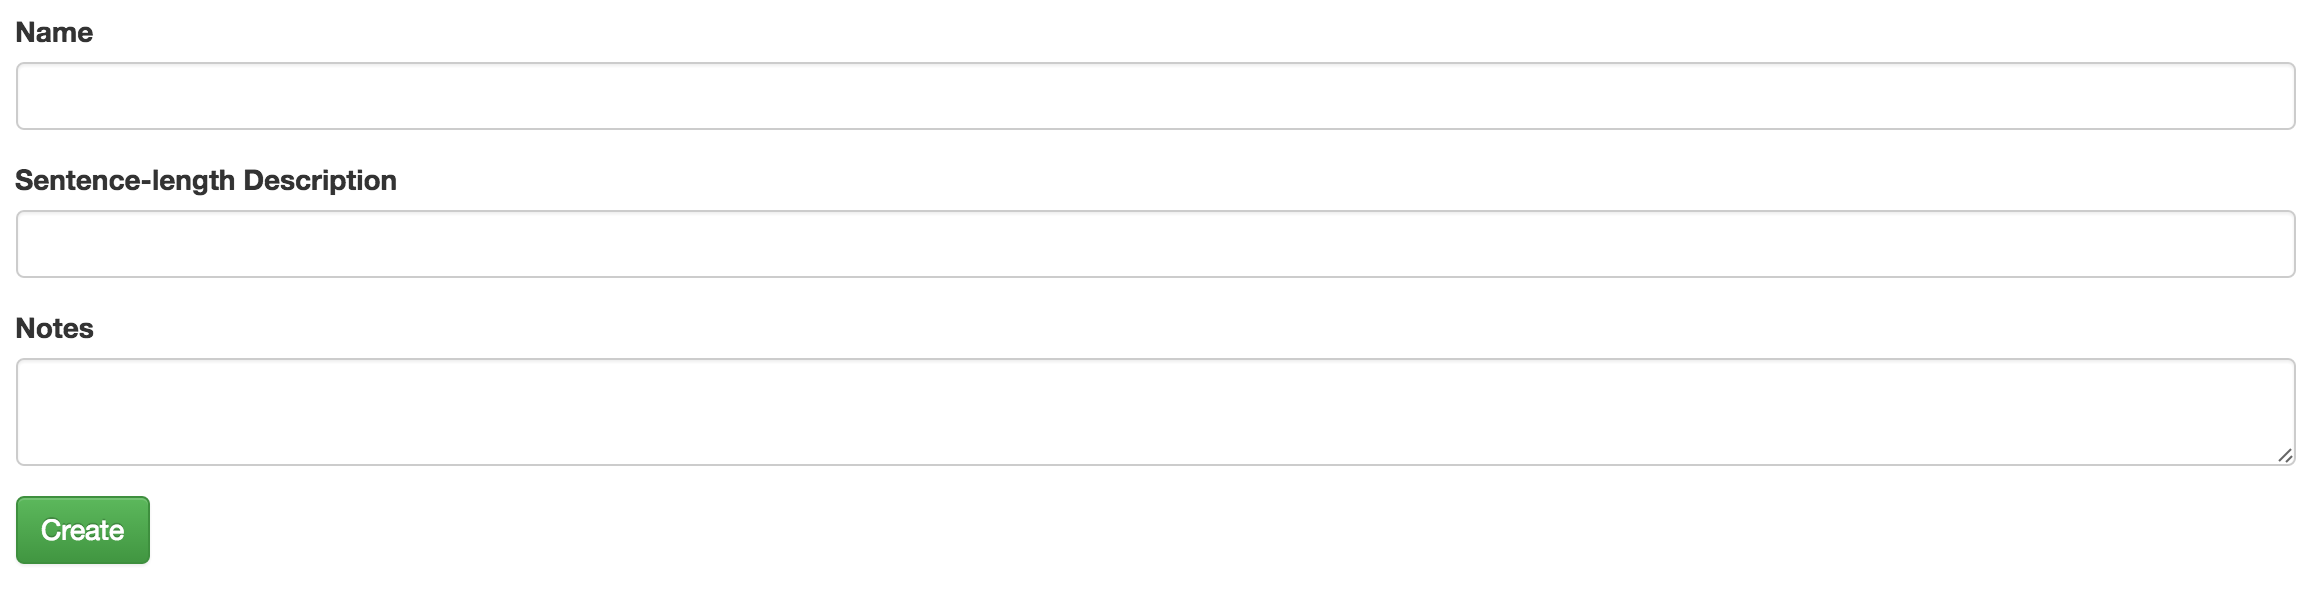
\includegraphics[width=\textwidth]{figures/create-language}
\caption{The language creation form.}
\centering
\label{fig:create-language}
\end{figure}

To create a language, a user must provide some name for that language and a sentence-length description of that language. They can optionally provide notes about that language, though the usage of the notes section varies widely by user.

Once a user submits that form, they are taken to a very empty version of Figure \ref{fig:keebouuzhodee-not-logged-in}, but with controls to manipulate the language. These controls appear because the user is logged in. The empty language with controls can be see in Figure \ref{fig:empty-language-logged-in}.

\begin{figure}[h]
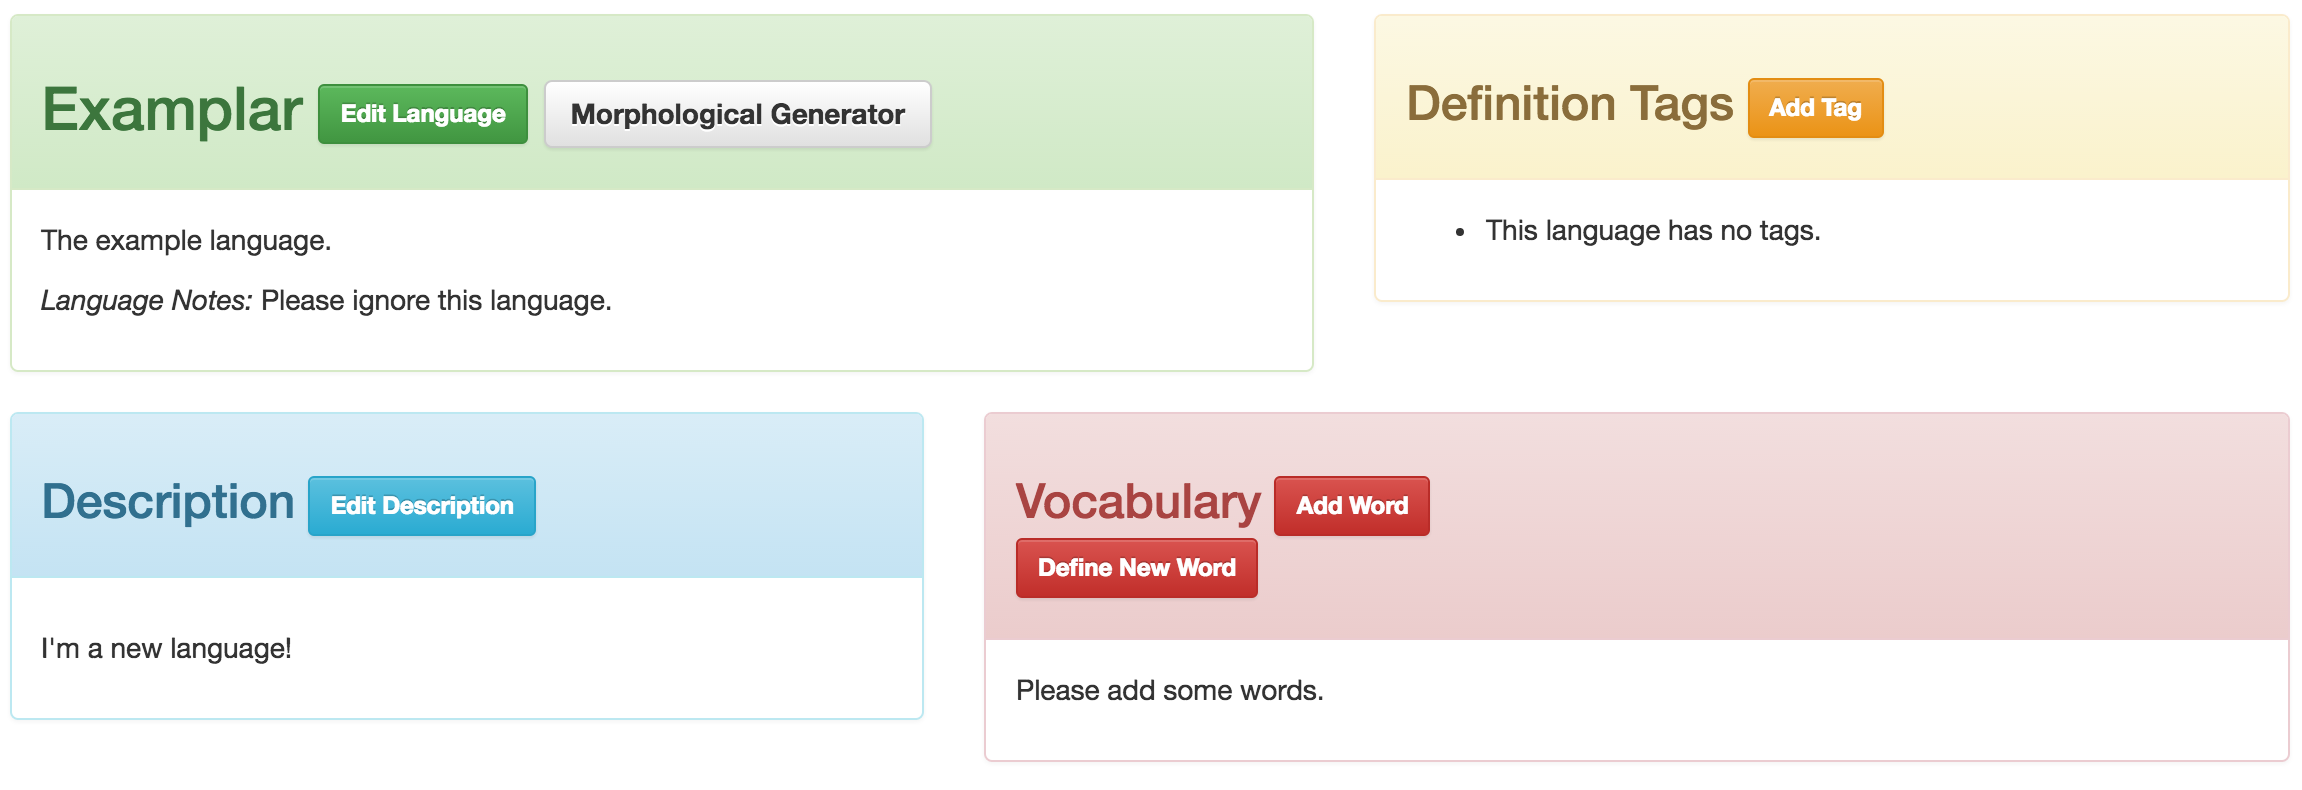
\includegraphics[width=\textwidth]{figures/empty-language-logged-in}
\caption{An empty language.}
\centering
\label{fig:empty-language-logged-in}
\end{figure}

\section{Defining a Word}
\label{sec:define-word}

Languages are built of words, and every word in a language has at least one meaning. To create a word with its first definition, a user can click the red ``Define New Word" button in Figure \ref{fig:empty-language-logged-in}. This will take a user to the form for creating words, which can be seen in Figure \ref{fig:define-word}.

\begin{figure}[h]
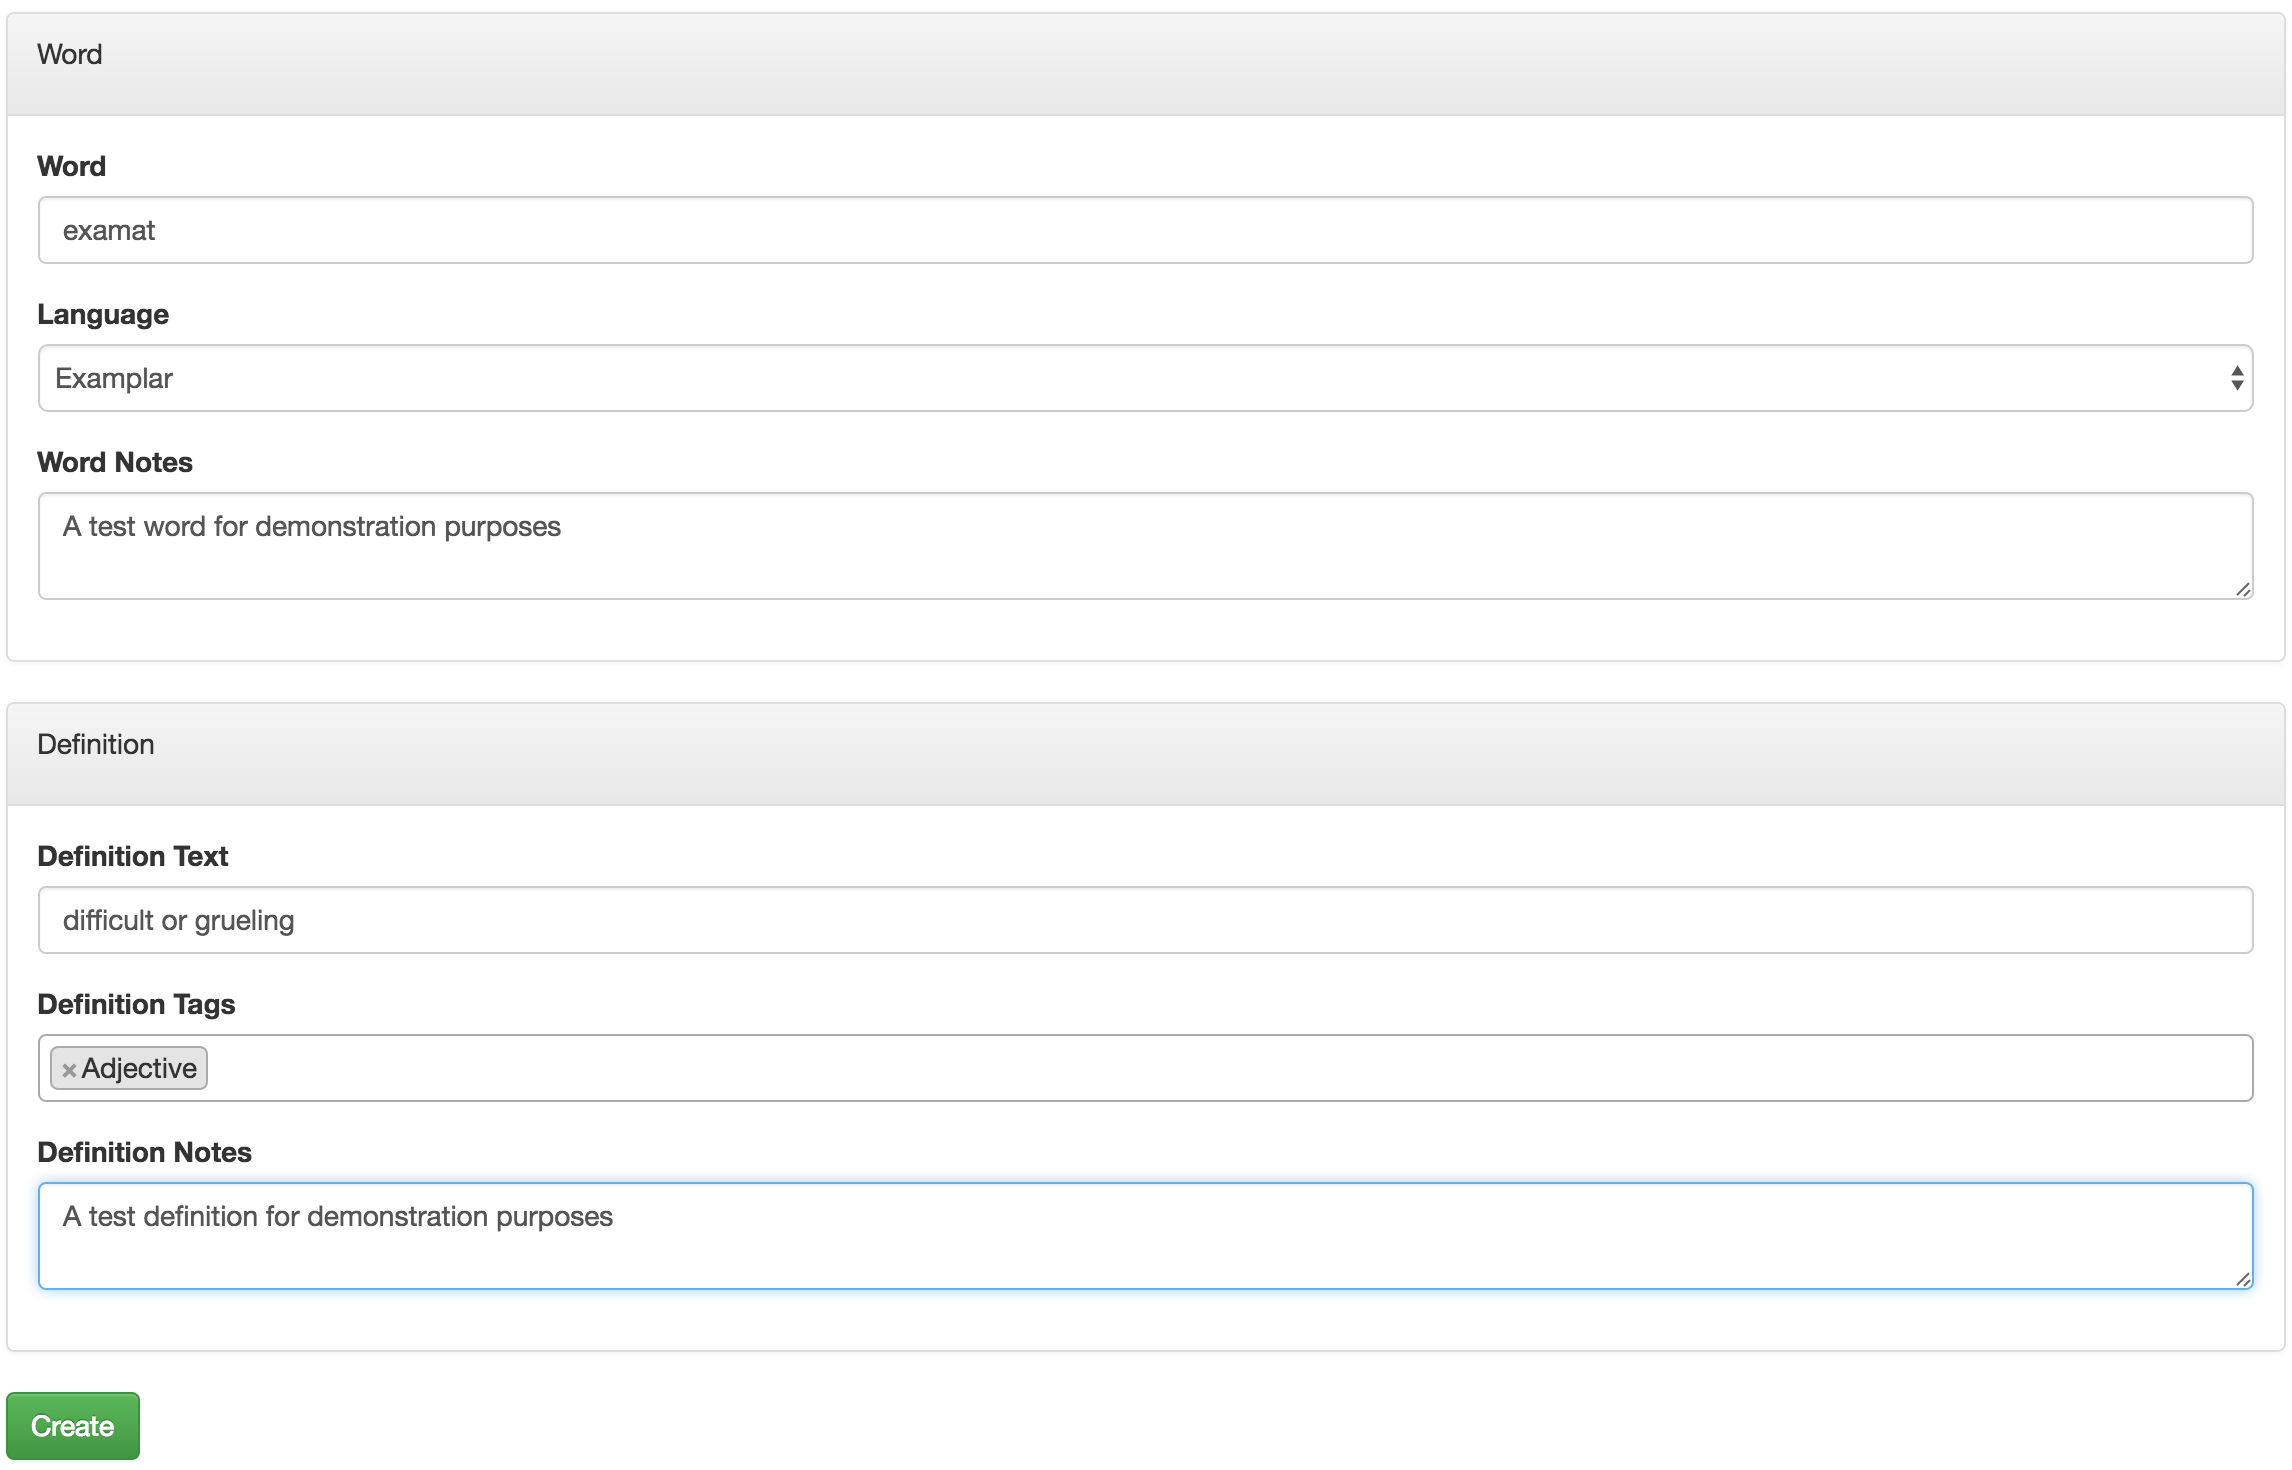
\includegraphics[width=\textwidth]{figures/define-word-filled-in}
\caption{The word definition form.}
\centering
\label{fig:define-word}
\end{figure}

The different form fields are fairly simple. The field labeled ``Word" is looking for the unicode string that this language uses to write down that word. The ``Language" dropdown menu allows a user to change which langauge that they are editing from this form, although this use case has become less and less common as the site has developed. ``Word Notes" can be any text regarding this word. These notes are intended to be a place for conlangers to discuss this word with one another.

The Definition section of the form is used to create this word's first definition. ``Definition Text" is the actual phrase or sentence describing the meaning of the word in a given context. ``Definition Tags" is an input for adding multiple tags to a word. If a user clicks within the ``Definition Tags" form field, it will bring up a dropdown menu of every tag in the language. The user can select as many or as few tags as they wish to. Additionally, typing the name of a new tag and pressing the Enter (or Return) key will create a new Tag in the language that will be attached to this definition. ``Definition Notes" serve the same role as Word Notes, but regarding a specific definition instead of a word.

\begin{figure}[h]
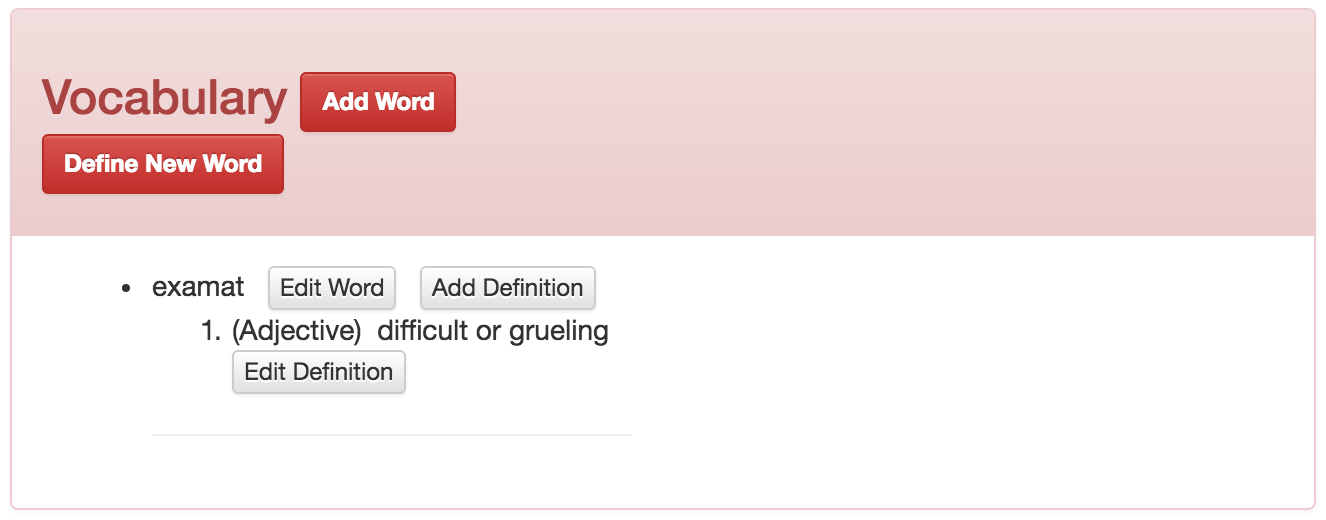
\includegraphics[width=\textwidth]{figures/example-language-one-word-logged-in}
\caption{An example language with its first word and definition.}
\centering
\label{fig:example-language-one-word-logged-in}
\end{figure}

When the user submits this form, they will be returned to the language's page, but it will now contain
their word and definition (see Figure \ref{fig:example-language-one-word-logged-in}).

\section{Creating a Definition}
\label{sec:create-definition}

Once you have a word, adding a definition is straightforward. The ``Add Definition" button in Figure \ref{fig:example-language-one-word-logged-in} takes a user to the definition creation form. The definition creation form has the exact same components as the definition section of Figure \ref{fig:define-word}, and it can be filled out in the same way.

Editing a definition uses this same form. To edit a definition, use the ``Edit Definition" button next to the definition in question in Figure \ref{fig:example-language-one-word-logged-in}.

\section{Creating a Tag}
\label{sec:create-tag}

Creating a tag works much the same way as creating a definition. Using the yellow ``Add Tag" button in Figure \ref{fig:empty-language-logged-in}, a user can access the tag creation form (Figure \ref{fig:create-tag}). 

\begin{figure}[h]
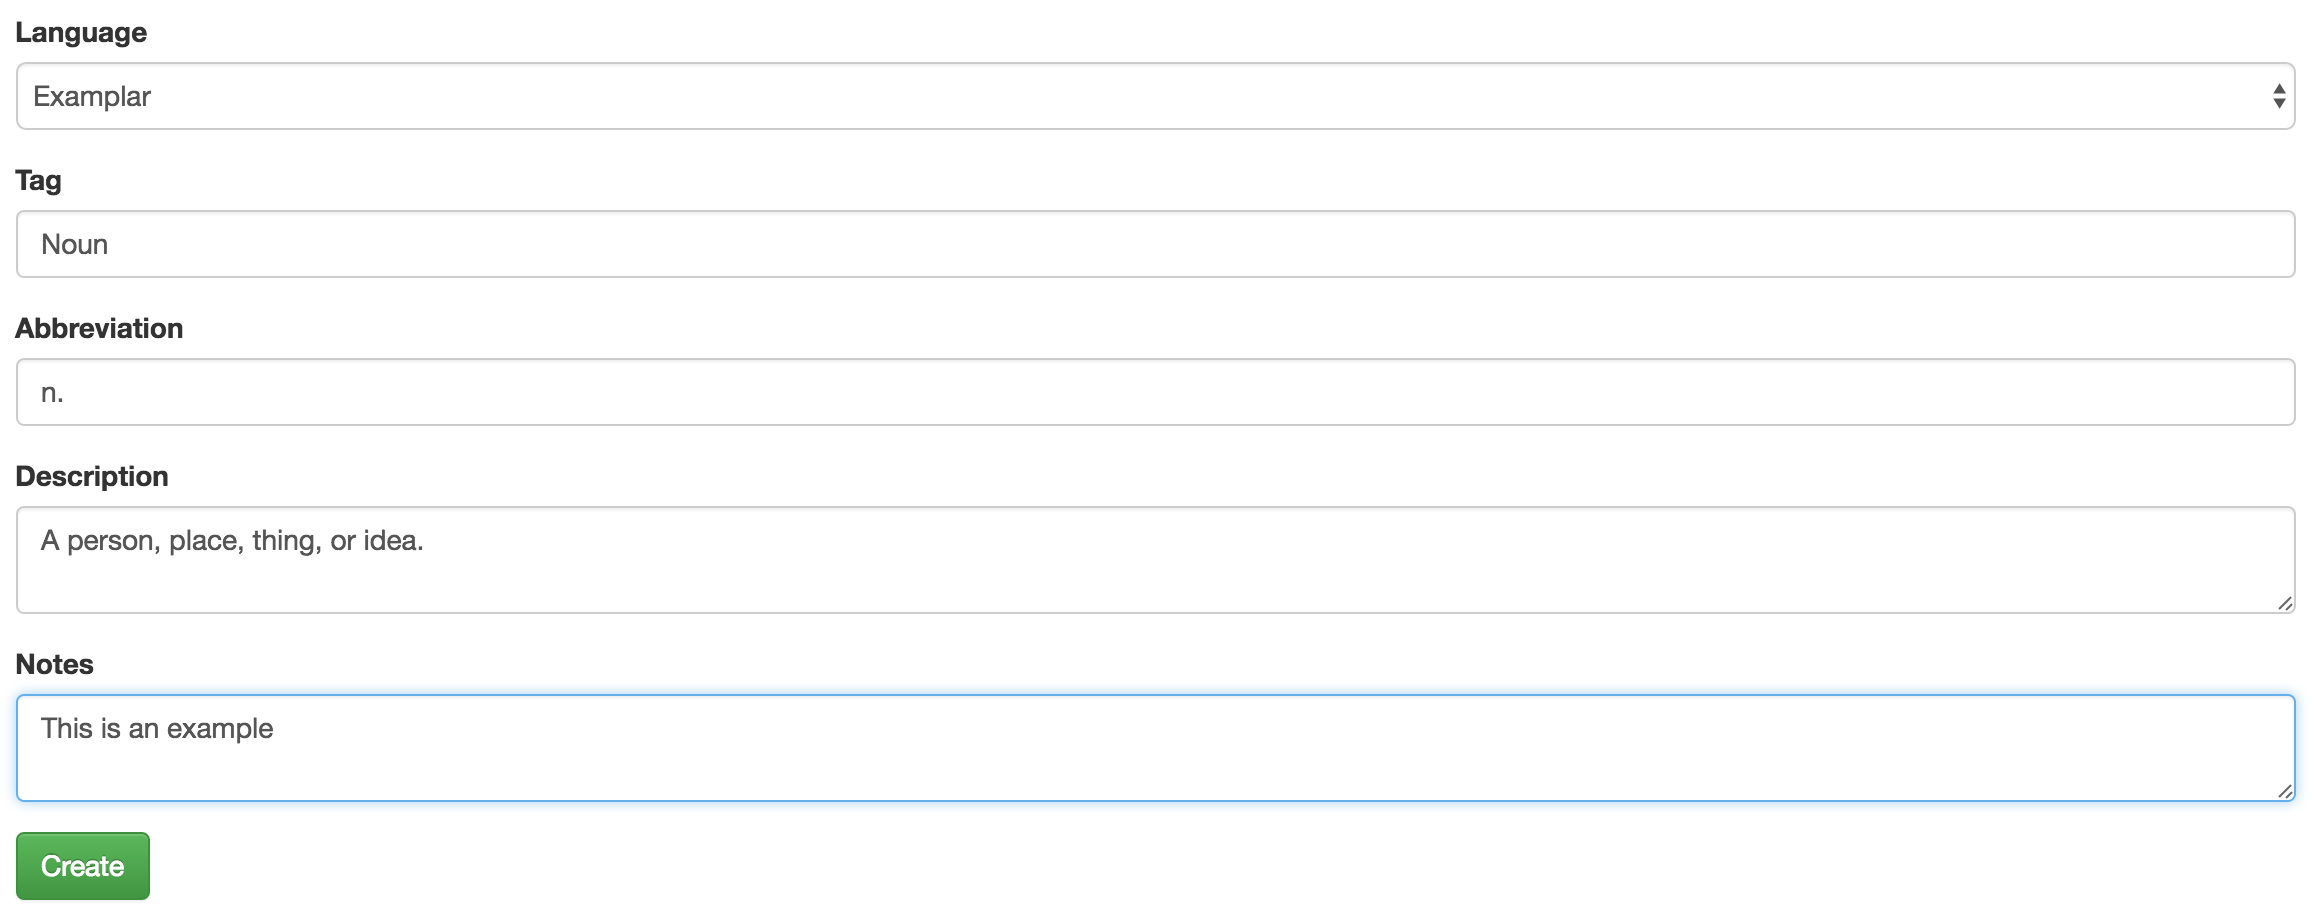
\includegraphics[width=\textwidth]{figures/create-tag}
\caption{The tag creation form.}
\centering
\label{fig:create-tag}
\end{figure}

The tag needs a name. Since tags can be used to encode any kind of information about a definition, it is difficult to suggest what to use. If a user is encoding parts of speech, the name of that part of speech will suffice. 

Tags also ask for an abbreviation. This will be displayed before the definition text of any definition with that tag. For parts of speech, this makes it very easy to display (n.) before nouns and so forth.

The tag description is a text description of what it means for a word to bear that tag. For parts of speech this can be a description of the role of that part of speech, but for other kinds of tag this can become quite complex. For instance, if a user were to tag by verb conjugation type, the description would need to explain how that type conjugates, or at least the difference between words in that class of conjugation and other words in the language.

As with every data entity in Conlangtionary, tags can also have notes, which ought to be used for internal reference and collaboration on the part of conlangers working with the language.

\section{Editing the Description}
\label{sec:edit-description}

The language description is simply a text area that supports the Markdown text format \cite{Markdown}. Users can write any content related to the language that they desire. Because it uses Markdown, users can even provide links to external resources about their languages if they desire.

The form looks like Figure \ref{fig:edit-description}, and it provides a link to resources on Markdown for users who might be unfamiliar with the format.

\begin{figure}[h]
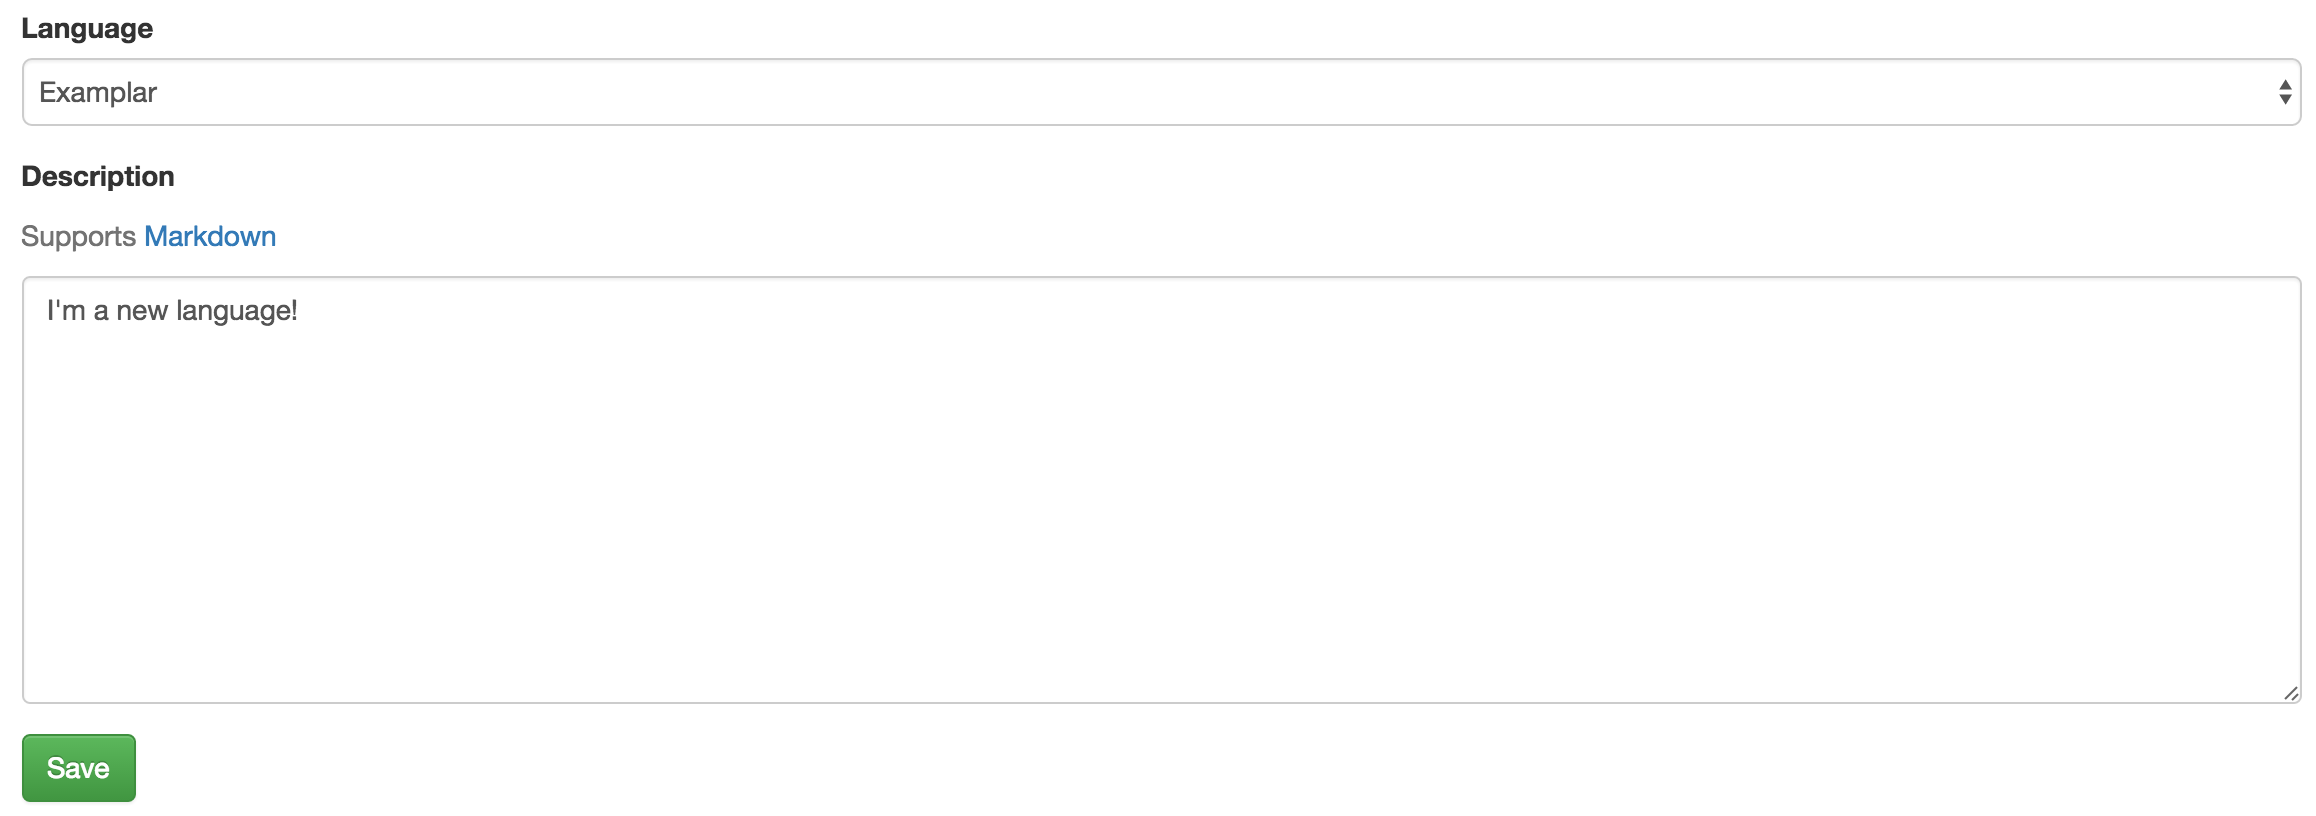
\includegraphics[width=\textwidth]{figures/edit-description}
\caption{The description editing form.}
\centering
\label{fig:edit-description}
\end{figure}

\section{Using the Morphological Generator}
\label{sec:using-morph-gen}

The Morphological Generator is the real power tool at the heart of Conlangtionary. Without it, Conlangtionary as a platform is just a descriptive tool. With it, Conlangtionary becomes a generative tool in its own right.

Morphological Generation is all about transforming a word from one form to another. To start with, Conlangtionary assumes that the word (or, more accurately, the word's definition) is tagged with all of the necessary information to distinguish between words that should be transformed and words that should not be affected. If definitions are not tagged with sufficient granularity, the generator will be useless for that language.

For example, if a user has tagged all of the Adjectives in a language simply as Adjectives, they could easily transform adjectives into a noun form \textit{if} all adjectives morph into nouns following a single, consistent rule. For the sake of a simple example, assume that the language in question is called SIMPLE and has the rule that any adjective can be made into a noun by adding the suffix ``ack." To turn the made-up SIMPLE adjective ``yasson" into a noun, one simply makes it ``yassonack." To perform this change, a user can simply tell Conlangtionary to take all definitions in SIMPLE with the tag ``Adjective" and add ``-ack" to the end of their word forms to create new words with the same definition as the Adjectives but tagged as ``Noun". If that rule has exceptions, then the generator cannot be applied unless all of the words that follow the rule share an additional tag that the words that do not follow the rule lack. If all of the adjectives that follow the rule share the tag ``Regularly-Nominalized," the generator can still perform the transformation. The only difference would be that it must select definitions bearing both the ``Adjective" tag and the ``Regularly-Nominalized" tag.

To specify this transformation through the user interface, a user must click the gray ``Morphological Generator" button seen in Figure \ref{fig:empty-language-logged-in}. This will bring a user to the page shown in Figure \ref{fig:morphological-generator}.

\begin{figure}[h]
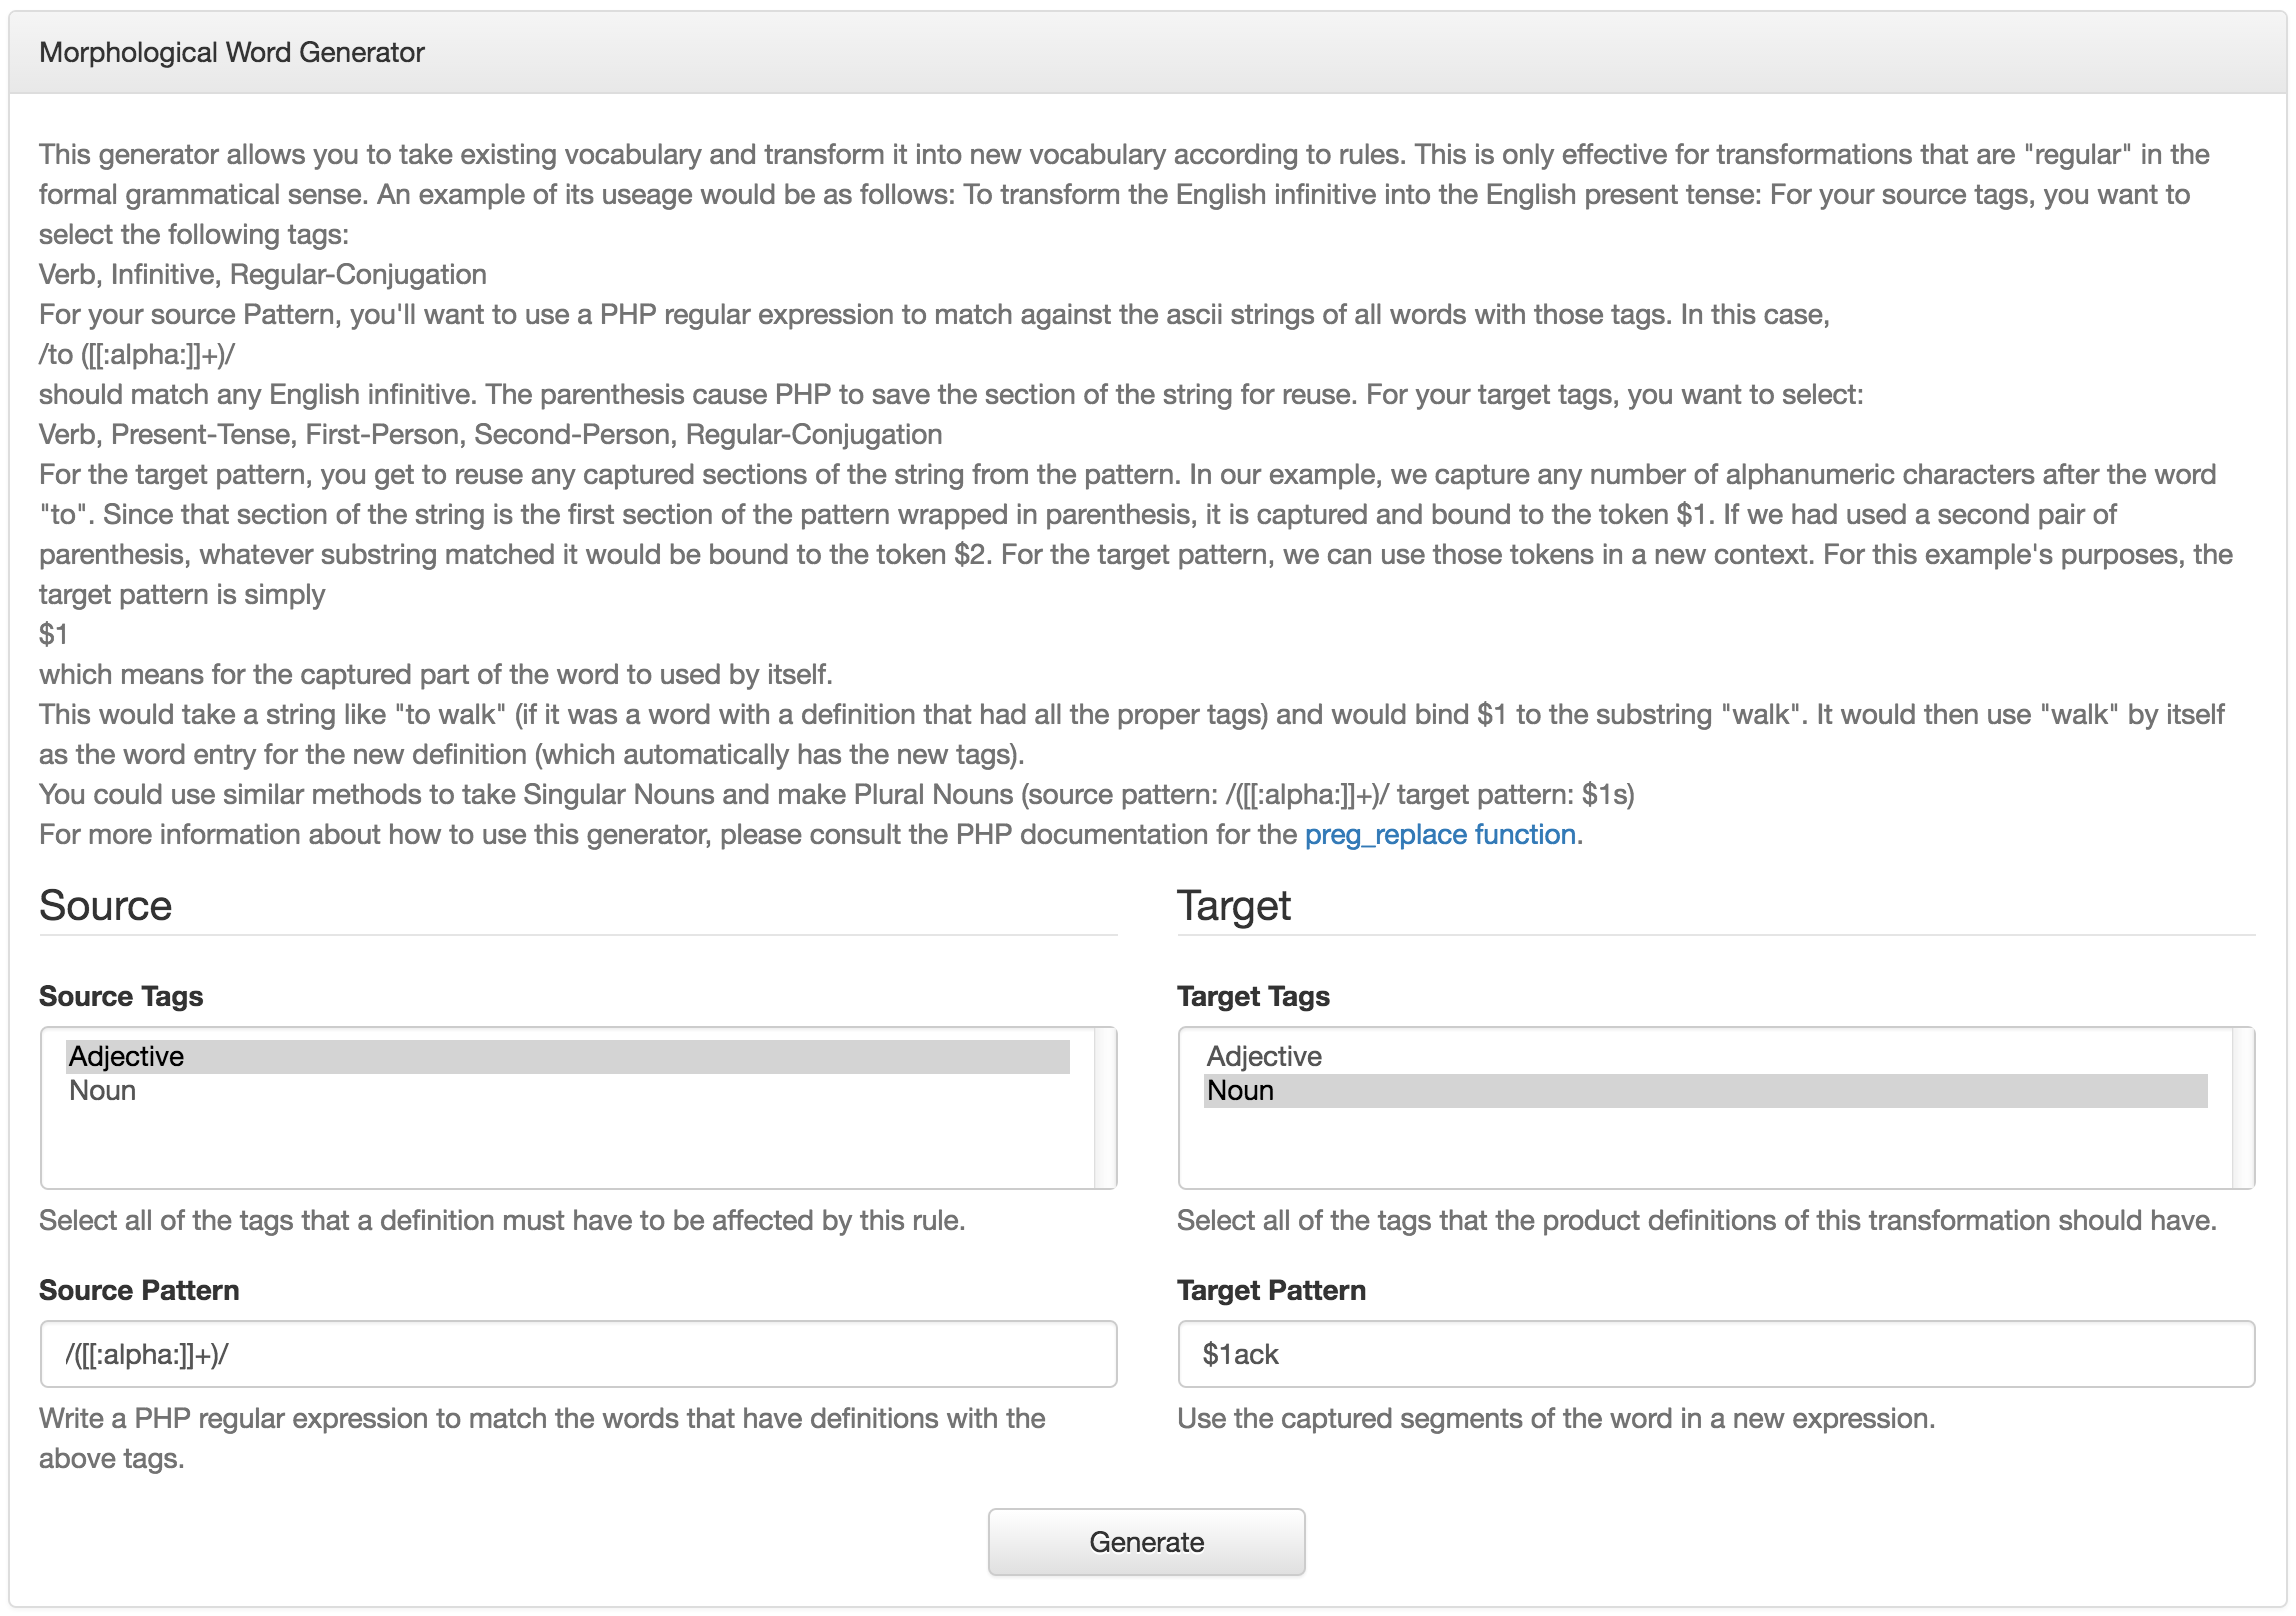
\includegraphics[width=\textwidth]{figures/morphological-generator-filled-in}
\caption{The morphological generator.}
\centering
\label{fig:morphological-generator}
\end{figure}

There is an explanation of the use of the generator on the page, but another is included here for the sake of completeness.

First, a user should select the tags that they want to operate on from the ``Source Tags" multi-select form element on the left. To select more than one, hold down the control key when clicking. Once the source tags have been chosen, the user should insert a PHP regular expression into the ``Source Pattern" input. This pattern is used to recognize and capture parts of the words that are needed in the result of the transformation. In the case of the above example, the user would select Adjective as a source tag and would use the pattern \url{/^([[:alpha:]]+)$/} to capture the entire word as an adjective.

After configuring the source information, the user follows a similar procedure to specify the output of the transformation. ``Target Tags" are the tags that the definitions created by the generator will bear, and ``Target Pattern" specifies the structure of the words that those definitions will define. To continue with the same example, the target tag would be ``Noun" and the target pattern would be \url{$1ack}. The ``\$1" is replaced with the first item from the source pattern that was surrounded by parenthesis. Since the source pattern surrounds the whole word with parenthesis, the target pattern will append ``ack" to the source words and define them tagged as nouns instead of adjectives. The definitions may need to be rephrased to reflect that the words have changed parts of speech, but such changes are too subtle to be automated.

Once a user clicks ``Generate," Conlangtionary will transform all matching words and insert them with the same definitions text that they had before. The difference will be that the definitions will bear different tags. While this may not seem exceedingly useful in the above instance because the user might need to rewrite dozens of definitions, it can very easily be used to generate alternative conjugations of a verb or declensions of a noun without needing to change any definition text.